\documentclass[1p]{elsarticle_modified}
%\bibliographystyle{elsarticle-num}

%\usepackage[colorlinks]{hyperref}
%\usepackage{abbrmath_seonhwa} %\Abb, \Ascr, \Acal ,\Abf, \Afrak
\usepackage{amsfonts}
\usepackage{amssymb}
\usepackage{amsmath}
\usepackage{amsthm}
\usepackage{scalefnt}
\usepackage{amsbsy}
\usepackage{kotex}
\usepackage{caption}
\usepackage{subfig}
\usepackage{color}
\usepackage{graphicx}
\usepackage{xcolor} %% white, black, red, green, blue, cyan, magenta, yellow
\usepackage{float}
\usepackage{setspace}
\usepackage{hyperref}

\usepackage{tikz}
\usetikzlibrary{arrows}

\usepackage{multirow}
\usepackage{array} % fixed length table
\usepackage{hhline}

%%%%%%%%%%%%%%%%%%%%%
\makeatletter
\renewcommand*\env@matrix[1][\arraystretch]{%
	\edef\arraystretch{#1}%
	\hskip -\arraycolsep
	\let\@ifnextchar\new@ifnextchar
	\array{*\c@MaxMatrixCols c}}
\makeatother %https://tex.stackexchange.com/questions/14071/how-can-i-increase-the-line-spacing-in-a-matrix
%%%%%%%%%%%%%%%

\usepackage[normalem]{ulem}

\newcommand{\msout}[1]{\ifmmode\text{\sout{\ensuremath{#1}}}\else\sout{#1}\fi}
%SOURCE: \msout is \stkout macro in https://tex.stackexchange.com/questions/20609/strikeout-in-math-mode

\newcommand{\cancel}[1]{
	\ifmmode
	{\color{red}\msout{#1}}
	\else
	{\color{red}\sout{#1}}
	\fi
}

\newcommand{\add}[1]{
	{\color{blue}\uwave{#1}}
}

\newcommand{\replace}[2]{
	\ifmmode
	{\color{red}\msout{#1}}{\color{blue}\uwave{#2}}
	\else
	{\color{red}\sout{#1}}{\color{blue}\uwave{#2}}
	\fi
}

\newcommand{\Sol}{\mathcal{S}} %segment
\newcommand{\D}{D} %diagram
\newcommand{\A}{\mathcal{A}} %arc


%%%%%%%%%%%%%%%%%%%%%%%%%%%%%5 test

\def\sl{\operatorname{\textup{SL}}(2,\Cbb)}
\def\psl{\operatorname{\textup{PSL}}(2,\Cbb)}
\def\quan{\mkern 1mu \triangleright \mkern 1mu}

\theoremstyle{definition}
\newtheorem{thm}{Theorem}[section]
\newtheorem{prop}[thm]{Proposition}
\newtheorem{lem}[thm]{Lemma}
\newtheorem{ques}[thm]{Question}
\newtheorem{cor}[thm]{Corollary}
\newtheorem{defn}[thm]{Definition}
\newtheorem{exam}[thm]{Example}
\newtheorem{rmk}[thm]{Remark}
\newtheorem{alg}[thm]{Algorithm}

\newcommand{\I}{\sqrt{-1}}
\begin{document}

%\begin{frontmatter}
%
%\title{Boundary parabolic representations of knots up to 8 crossings}
%
%%% Group authors per affiliation:
%\author{Yunhi Cho} 
%\address{Department of Mathematics, University of Seoul, Seoul, Korea}
%\ead{yhcho@uos.ac.kr}
%
%
%\author{Seonhwa Kim} %\fnref{s_kim}}
%\address{Center for Geometry and Physics, Institute for Basic Science, Pohang, 37673, Korea}
%\ead{ryeona17@ibs.re.kr}
%
%\author{Hyuk Kim}
%\address{Department of Mathematical Sciences, Seoul National University, Seoul 08826, Korea}
%\ead{hyukkim@snu.ac.kr}
%
%\author{Seokbeom Yoon}
%\address{Department of Mathematical Sciences, Seoul National University, Seoul, 08826,  Korea}
%\ead{sbyoon15@snu.ac.kr}
%
%\begin{abstract}
%We find all boundary parabolic representation of knots up to 8 crossings.
%
%\end{abstract}
%\begin{keyword}
%    \MSC[2010] 57M25 
%\end{keyword}
%
%\end{frontmatter}

%\linenumbers
%\tableofcontents
%
\newcommand\colored[1]{\textcolor{white}{\rule[-0.35ex]{0.8em}{1.4ex}}\kern-0.8em\color{red} #1}%
%\newcommand\colored[1]{\textcolor{white}{ #1}\kern-2.17ex	\textcolor{white}{ #1}\kern-1.81ex	\textcolor{white}{ #1}\kern-2.15ex\color{red}#1	}

{\Large $\underline{12a_{0239}~(K12a_{0239})}$}

\setlength{\tabcolsep}{10pt}
\renewcommand{\arraystretch}{1.6}
\vspace{1cm}\begin{tabular}{m{100pt}>{\centering\arraybackslash}m{274pt}}
\multirow{5}{120pt}{
	\centering
	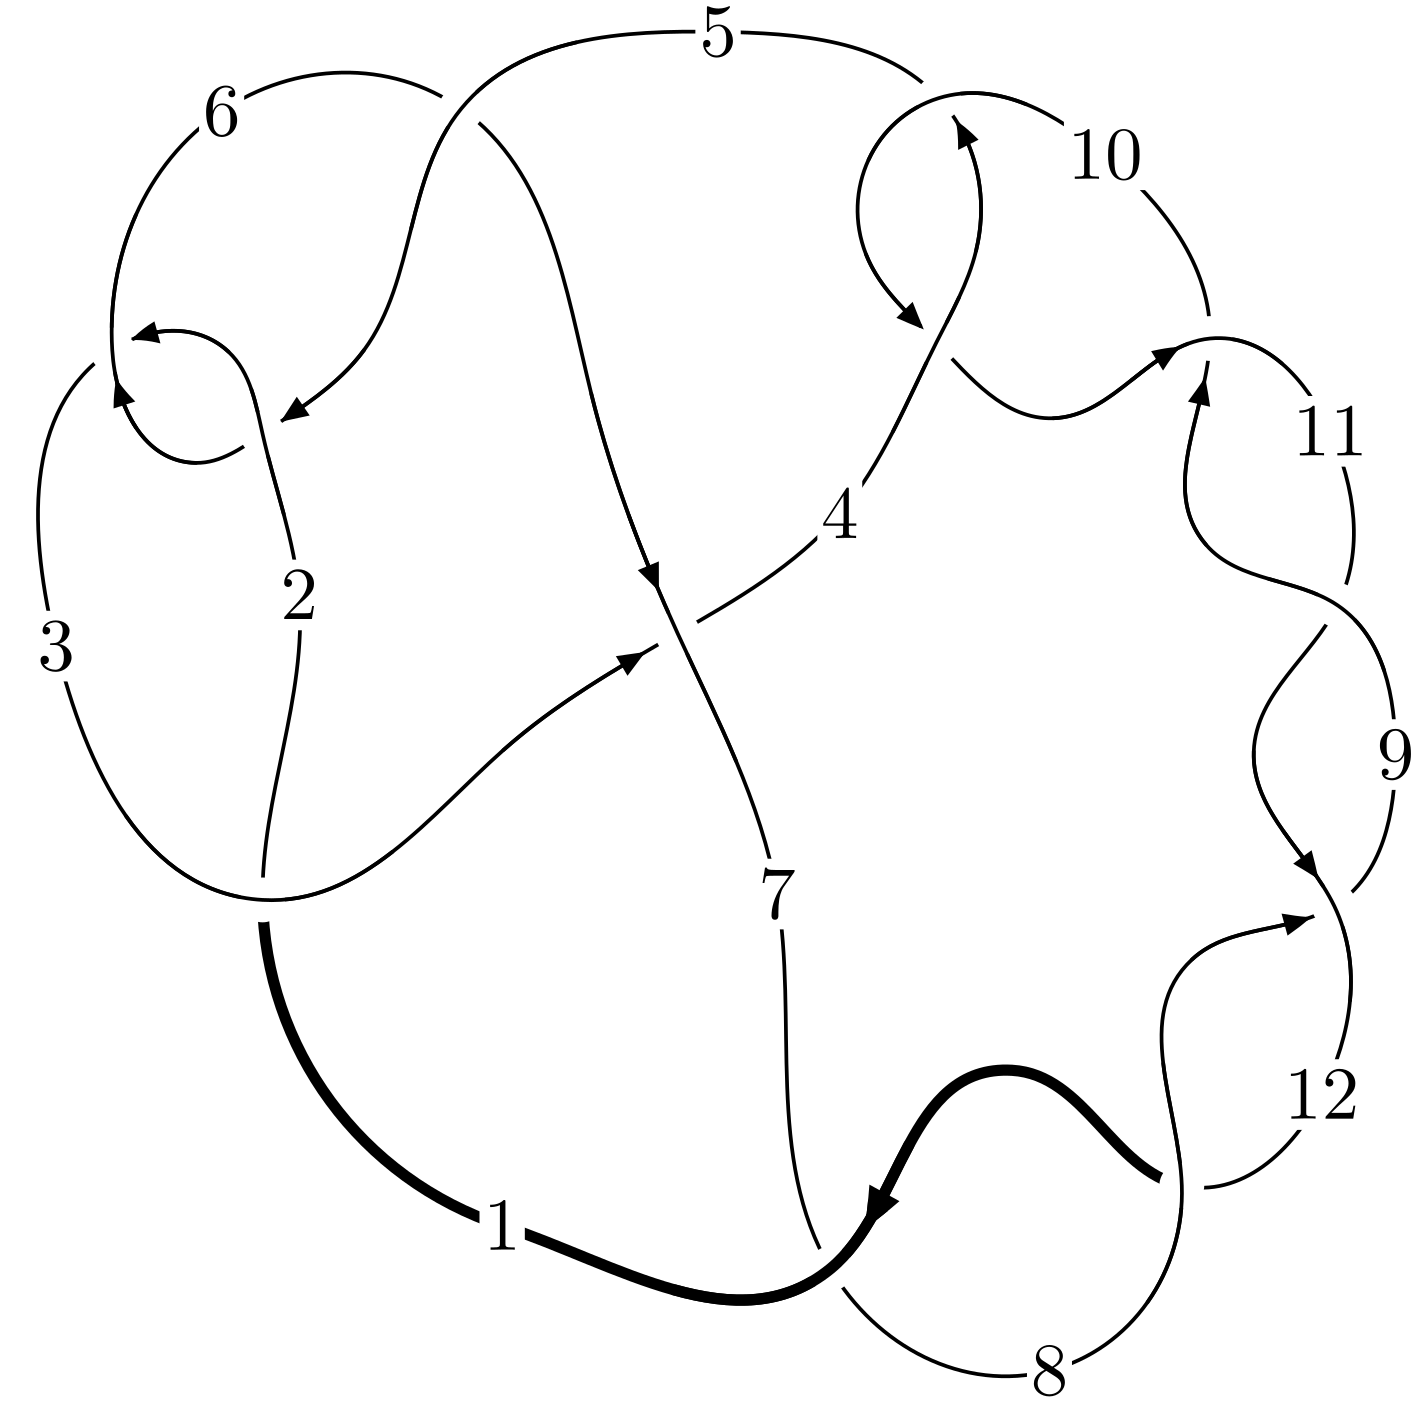
\includegraphics[width=112pt]{../../../GIT/diagram.site/Diagrams/png/1040_12a_0239.png}\\
\ \ \ A knot diagram\footnotemark}&
\allowdisplaybreaks
\textbf{Linearized knot diagam} \\
\cline{2-2}
 &
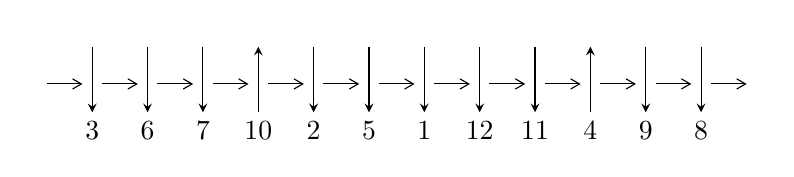
\begin{tikzpicture}[x=20pt, y=17pt]
	% nodes
	\node (C0) at (0, 0) {};
	\node (C1) at (1, 0) {};
	\node (C1U) at (1, +1) {};
	\node (C1D) at (1, -1) {3};

	\node (C2) at (2, 0) {};
	\node (C2U) at (2, +1) {};
	\node (C2D) at (2, -1) {6};

	\node (C3) at (3, 0) {};
	\node (C3U) at (3, +1) {};
	\node (C3D) at (3, -1) {7};

	\node (C4) at (4, 0) {};
	\node (C4U) at (4, +1) {};
	\node (C4D) at (4, -1) {10};

	\node (C5) at (5, 0) {};
	\node (C5U) at (5, +1) {};
	\node (C5D) at (5, -1) {2};

	\node (C6) at (6, 0) {};
	\node (C6U) at (6, +1) {};
	\node (C6D) at (6, -1) {5};

	\node (C7) at (7, 0) {};
	\node (C7U) at (7, +1) {};
	\node (C7D) at (7, -1) {1};

	\node (C8) at (8, 0) {};
	\node (C8U) at (8, +1) {};
	\node (C8D) at (8, -1) {12};

	\node (C9) at (9, 0) {};
	\node (C9U) at (9, +1) {};
	\node (C9D) at (9, -1) {11};

	\node (C10) at (10, 0) {};
	\node (C10U) at (10, +1) {};
	\node (C10D) at (10, -1) {4};

	\node (C11) at (11, 0) {};
	\node (C11U) at (11, +1) {};
	\node (C11D) at (11, -1) {9};

	\node (C12) at (12, 0) {};
	\node (C12U) at (12, +1) {};
	\node (C12D) at (12, -1) {8};
	\node (C13) at (13, 0) {};

	% arrows
	\draw[->,>={angle 60}]
	(C0) edge (C1) (C1) edge (C2) (C2) edge (C3) (C3) edge (C4) (C4) edge (C5) (C5) edge (C6) (C6) edge (C7) (C7) edge (C8) (C8) edge (C9) (C9) edge (C10) (C10) edge (C11) (C11) edge (C12) (C12) edge (C13) ;	\draw[->,>=stealth]
	(C1U) edge (C1D) (C2U) edge (C2D) (C3U) edge (C3D) (C4D) edge (C4U) (C5U) edge (C5D) (C6U) edge (C6D) (C7U) edge (C7D) (C8U) edge (C8D) (C9U) edge (C9D) (C10D) edge (C10U) (C11U) edge (C11D) (C12U) edge (C12D) ;
	\end{tikzpicture} \\
\hhline{~~} \\& 
\textbf{Solving Sequence} \\ \cline{2-2} 
 &
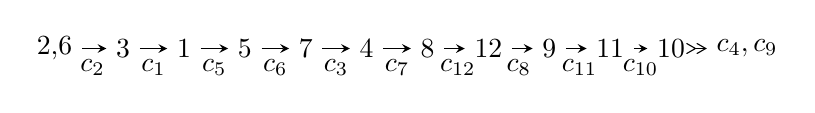
\begin{tikzpicture}[x=22pt, y=7pt]
	% node
	\node (A0) at (-1/8, 0) {2,6};
	\node (A1) at (1, 0) {3};
	\node (A2) at (2, 0) {1};
	\node (A3) at (3, 0) {5};
	\node (A4) at (4, 0) {7};
	\node (A5) at (5, 0) {4};
	\node (A6) at (6, 0) {8};
	\node (A7) at (7, 0) {12};
	\node (A8) at (8, 0) {9};
	\node (A9) at (9, 0) {11};
	\node (A10) at (10, 0) {10};
	\node (C1) at (1/2, -1) {$c_{2}$};
	\node (C2) at (3/2, -1) {$c_{1}$};
	\node (C3) at (5/2, -1) {$c_{5}$};
	\node (C4) at (7/2, -1) {$c_{6}$};
	\node (C5) at (9/2, -1) {$c_{3}$};
	\node (C6) at (11/2, -1) {$c_{7}$};
	\node (C7) at (13/2, -1) {$c_{12}$};
	\node (C8) at (15/2, -1) {$c_{8}$};
	\node (C9) at (17/2, -1) {$c_{11}$};
	\node (C10) at (19/2, -1) {$c_{10}$};
	\node (A11) at (45/4, 0) {$c_{4},c_{9}$};

	% edge
	\draw[->,>=stealth]	
	(A0) edge (A1) (A1) edge (A2) (A2) edge (A3) (A3) edge (A4) (A4) edge (A5) (A5) edge (A6) (A6) edge (A7) (A7) edge (A8) (A8) edge (A9) (A9) edge (A10) ;
	\draw[->>,>={angle 60}]	
	(A10) edge (A11);
\end{tikzpicture} \\ 

\end{tabular} \\

\footnotetext{
The image of knot diagram is generated by the software ``\textbf{Draw programme}" developed by Andrew Bartholomew(\url{http://www.layer8.co.uk/maths/draw/index.htm\#Running-draw}), where we modified some parts for our purpose(\url{https://github.com/CATsTAILs/LinksPainter}).
}\phantom \\ \newline 
\centering \textbf{Ideals for irreducible components\footnotemark of $X_{\text{par}}$} 
 
\begin{align*}
I^u_{1}&=\langle 
u^{43}+u^{42}+\cdots+4 u+1\rangle \\
\\
\end{align*}
\raggedright * 1 irreducible components of $\dim_{\mathbb{C}}=0$, with total 43 representations.\\
\footnotetext{All coefficients of polynomials are rational numbers. But the coefficients are sometimes approximated in decimal forms when there is not enough margin.}
\newpage
\renewcommand{\arraystretch}{1}
\centering \section*{I. $I^u_{1}= \langle u^{43}+u^{42}+\cdots+4 u+1 \rangle$}
\flushleft \textbf{(i) Arc colorings}\\
\begin{tabular}{m{7pt} m{180pt} m{7pt} m{180pt} }
\flushright $a_{2}=$&$\begin{pmatrix}1\\0\end{pmatrix}$ \\
\flushright $a_{6}=$&$\begin{pmatrix}0\\u\end{pmatrix}$ \\
\flushright $a_{3}=$&$\begin{pmatrix}1\\u^2\end{pmatrix}$ \\
\flushright $a_{1}=$&$\begin{pmatrix}- u^2+1\\- u^4\end{pmatrix}$ \\
\flushright $a_{5}=$&$\begin{pmatrix}u\\u\end{pmatrix}$ \\
\flushright $a_{7}=$&$\begin{pmatrix}- u^3\\- u^3+u\end{pmatrix}$ \\
\flushright $a_{4}=$&$\begin{pmatrix}- u^8+u^6- u^4+1\\- u^8+2 u^6-2 u^4+2 u^2\end{pmatrix}$ \\
\flushright $a_{8}=$&$\begin{pmatrix}- u^9+2 u^7-3 u^5+2 u^3- u\\- u^{11}+u^9-2 u^7+u^5- u^3+u\end{pmatrix}$ \\
\flushright $a_{12}=$&$\begin{pmatrix}- u^{16}+3 u^{14}-7 u^{12}+10 u^{10}-11 u^8+8 u^6-4 u^4+1\\- u^{18}+2 u^{16}-5 u^{14}+6 u^{12}-7 u^{10}+6 u^8-4 u^6+2 u^4- u^2\end{pmatrix}$ \\
\flushright $a_{9}=$&$\begin{pmatrix}- u^{23}+4 u^{21}+\cdots+4 u^3-2 u\\- u^{25}+3 u^{23}+\cdots-3 u^5+u\end{pmatrix}$ \\
\flushright $a_{11}=$&$\begin{pmatrix}- u^{30}+5 u^{28}+\cdots+2 u^2+1\\- u^{32}+4 u^{30}+\cdots+4 u^4-2 u^2\end{pmatrix}$ \\
\flushright $a_{10}=$&$\begin{pmatrix}- u^{37}+6 u^{35}+\cdots+4 u^3-3 u\\- u^{39}+5 u^{37}+\cdots+2 u^3+u\end{pmatrix}$\\&\end{tabular}
\flushleft \textbf{(ii) Obstruction class $= -1$}\\~\\
\flushleft \textbf{(iii) Cusp Shapes $= -4 u^{42}+28 u^{40}+\cdots-48 u-18$}\\~\\
\newpage\renewcommand{\arraystretch}{1}
\flushleft \textbf{(iv) u-Polynomials at the component}\newline \\
\begin{tabular}{m{50pt}|m{274pt}}
Crossings & \hspace{64pt}u-Polynomials at each crossing \\
\hline $$\begin{aligned}c_{1},c_{6}\end{aligned}$$&$\begin{aligned}
&u^{43}+13 u^{42}+\cdots-2 u+1
\end{aligned}$\\
\hline $$\begin{aligned}c_{2},c_{5}\end{aligned}$$&$\begin{aligned}
&u^{43}+u^{42}+\cdots+4 u+1
\end{aligned}$\\
\hline $$\begin{aligned}c_{3}\end{aligned}$$&$\begin{aligned}
&u^{43}- u^{42}+\cdots+1822 u+673
\end{aligned}$\\
\hline $$\begin{aligned}c_{4},c_{10}\end{aligned}$$&$\begin{aligned}
&u^{43}+u^{42}+\cdots+2 u+1
\end{aligned}$\\
\hline $$\begin{aligned}c_{7},c_{8},c_{9}\\c_{11},c_{12}\end{aligned}$$&$\begin{aligned}
&u^{43}+7 u^{42}+\cdots-2 u-1
\end{aligned}$\\
\hline
\end{tabular}\\~\\
\newpage\renewcommand{\arraystretch}{1}
\flushleft \textbf{(v) Riley Polynomials at the component}\newline \\
\begin{tabular}{m{50pt}|m{274pt}}
Crossings & \hspace{64pt}Riley Polynomials at each crossing \\
\hline $$\begin{aligned}c_{1},c_{6}\end{aligned}$$&$\begin{aligned}
&y^{43}+35 y^{42}+\cdots-58 y-1
\end{aligned}$\\
\hline $$\begin{aligned}c_{2},c_{5}\end{aligned}$$&$\begin{aligned}
&y^{43}-13 y^{42}+\cdots-2 y-1
\end{aligned}$\\
\hline $$\begin{aligned}c_{3}\end{aligned}$$&$\begin{aligned}
&y^{43}+23 y^{42}+\cdots-3215146 y-452929
\end{aligned}$\\
\hline $$\begin{aligned}c_{4},c_{10}\end{aligned}$$&$\begin{aligned}
&y^{43}+7 y^{42}+\cdots-2 y-1
\end{aligned}$\\
\hline $$\begin{aligned}c_{7},c_{8},c_{9}\\c_{11},c_{12}\end{aligned}$$&$\begin{aligned}
&y^{43}+59 y^{42}+\cdots+22 y-1
\end{aligned}$\\
\hline
\end{tabular}\\~\\
\newpage\flushleft \textbf{(vi) Complex Volumes and Cusp Shapes}
$$\begin{array}{c|c|c}  
\text{Solutions to }I^u_{1}& \I (\text{vol} + \sqrt{-1}CS) & \text{Cusp shape}\\
 \hline 
\begin{aligned}
u &= \phantom{-}0.981082 + 0.196833 I\end{aligned}
 & \phantom{-}0.87304 - 5.10243 I & -8.09536 + 7.65334 I \\ \hline\begin{aligned}
u &= \phantom{-}0.981082 - 0.196833 I\end{aligned}
 & \phantom{-}0.87304 + 5.10243 I & -8.09536 - 7.65334 I \\ \hline\begin{aligned}
u &= -0.756864 + 0.703321 I\end{aligned}
 & \phantom{-}1.54506 - 1.29052 I & -6.15207 + 4.41135 I \\ \hline\begin{aligned}
u &= -0.756864 - 0.703321 I\end{aligned}
 & \phantom{-}1.54506 + 1.29052 I & -6.15207 - 4.41135 I \\ \hline\begin{aligned}
u &= -0.929614 + 0.243471 I\end{aligned}
 & \phantom{-}1.314580 + 0.224610 I & -6.30893 - 0.94565 I \\ \hline\begin{aligned}
u &= -0.929614 - 0.243471 I\end{aligned}
 & \phantom{-}1.314580 - 0.224610 I & -6.30893 + 0.94565 I \\ \hline\begin{aligned}
u &= \phantom{-}0.944630 + 0.064820 I\end{aligned}
 & -3.51261 - 1.97345 I & -16.2504 + 5.9015 I \\ \hline\begin{aligned}
u &= \phantom{-}0.944630 - 0.064820 I\end{aligned}
 & -3.51261 + 1.97345 I & -16.2504 - 5.9015 I \\ \hline\begin{aligned}
u &= -1.043590 + 0.271851 I\end{aligned}
 & \phantom{-}10.99790 - 0.10309 I & -5.84751 - 1.12875 I \\ \hline\begin{aligned}
u &= -1.043590 - 0.271851 I\end{aligned}
 & \phantom{-}10.99790 + 0.10309 I & -5.84751 + 1.12875 I \\ \hline\begin{aligned}
u &= \phantom{-}1.047870 + 0.262426 I\end{aligned}
 & \phantom{-}10.93510 - 6.66217 I & -6.01718 + 5.66740 I \\ \hline\begin{aligned}
u &= \phantom{-}1.047870 - 0.262426 I\end{aligned}
 & \phantom{-}10.93510 + 6.66217 I & -6.01718 - 5.66740 I \\ \hline\begin{aligned}
u &= -0.881434 + 0.648427 I\end{aligned}
 & -0.47533 + 2.51394 I & -12.27687 - 2.56334 I \\ \hline\begin{aligned}
u &= -0.881434 - 0.648427 I\end{aligned}
 & -0.47533 - 2.51394 I & -12.27687 + 2.56334 I \\ \hline\begin{aligned}
u &= -0.740624 + 0.806639 I\end{aligned}
 & \phantom{-}7.37925 - 4.23077 I & -1.23707 + 3.77450 I \\ \hline\begin{aligned}
u &= -0.740624 - 0.806639 I\end{aligned}
 & \phantom{-}7.37925 + 4.23077 I & -1.23707 - 3.77450 I \\ \hline\begin{aligned}
u &= \phantom{-}0.829061 + 0.730502 I\end{aligned}
 & \phantom{-}3.10908 - 1.97013 I & -0.14053 + 3.02879 I \\ \hline\begin{aligned}
u &= \phantom{-}0.829061 - 0.730502 I\end{aligned}
 & \phantom{-}3.10908 + 1.97013 I & -0.14053 - 3.02879 I \\ \hline\begin{aligned}
u &= \phantom{-}0.768437 + 0.807890 I\end{aligned}
 & \phantom{-}7.89054 - 1.19457 I & \phantom{-}0.07490 + 2.40588 I \\ \hline\begin{aligned}
u &= \phantom{-}0.768437 - 0.807890 I\end{aligned}
 & \phantom{-}7.89054 + 1.19457 I & \phantom{-}0.07490 - 2.40588 I \\ \hline\begin{aligned}
u &= -0.743419 + 0.860690 I\end{aligned}
 & \phantom{-}18.3406 - 5.9453 I & -0.14706 + 2.39501 I \\ \hline\begin{aligned}
u &= -0.743419 - 0.860690 I\end{aligned}
 & \phantom{-}18.3406 + 5.9453 I & -0.14706 - 2.39501 I \\ \hline\begin{aligned}
u &= \phantom{-}0.748999 + 0.860570 I\end{aligned}
 & \phantom{-}18.4432 - 0.9130 I & \phantom{-0.000000 -}0. + 2.08674 I \\ \hline\begin{aligned}
u &= \phantom{-}0.748999 - 0.860570 I\end{aligned}
 & \phantom{-}18.4432 + 0.9130 I & \phantom{-0.000000 } 0. - 2.08674 I \\ \hline\begin{aligned}
u &= \phantom{-}0.908733 + 0.720344 I\end{aligned}
 & \phantom{-}2.86472 - 3.56465 I & -0.69891 + 3.15154 I \\ \hline\begin{aligned}
u &= \phantom{-}0.908733 - 0.720344 I\end{aligned}
 & \phantom{-}2.86472 + 3.56465 I & -0.69891 - 3.15154 I \\ \hline\begin{aligned}
u &= -0.949064 + 0.695827 I\end{aligned}
 & \phantom{-}0.96736 + 6.68062 I & -8.00000 - 9.76370 I \\ \hline\begin{aligned}
u &= -0.949064 - 0.695827 I\end{aligned}
 & \phantom{-}0.96736 - 6.68062 I & -8.00000 + 9.76370 I \\ \hline\begin{aligned}
u &= -0.820533\phantom{ +0.000000I}\end{aligned}
 & -1.33344\phantom{ +0.000000I} & -6.72830\phantom{ +0.000000I} \\ \hline\begin{aligned}
u &= \phantom{-}0.970139 + 0.751383 I\end{aligned}
 & \phantom{-}7.27360 - 4.66202 I & -1.06940 + 2.91522 I\\
 \hline 
 \end{array}$$\newpage$$\begin{array}{c|c|c}  
\text{Solutions to }I^u_{1}& \I (\text{vol} + \sqrt{-1}CS) & \text{Cusp shape}\\
 \hline 
\begin{aligned}
u &= \phantom{-}0.970139 - 0.751383 I\end{aligned}
 & \phantom{-}7.27360 + 4.66202 I & -1.06940 - 2.91522 I \\ \hline\begin{aligned}
u &= -0.984689 + 0.740034 I\end{aligned}
 & \phantom{-}6.63575 + 10.04490 I & -2.84536 - 8.98965 I \\ \hline\begin{aligned}
u &= -0.984689 - 0.740034 I\end{aligned}
 & \phantom{-}6.63575 - 10.04490 I & -2.84536 + 8.98965 I \\ \hline\begin{aligned}
u &= \phantom{-}1.004250 + 0.770086 I\end{aligned}
 & \phantom{-}17.6531 - 5.1564 I & -1.23638 + 2.77428 I \\ \hline\begin{aligned}
u &= \phantom{-}1.004250 - 0.770086 I\end{aligned}
 & \phantom{-}17.6531 + 5.1564 I & -1.23638 - 2.77428 I \\ \hline\begin{aligned}
u &= -1.007150 + 0.767415 I\end{aligned}
 & \phantom{-}17.5245 + 12.0059 I & -1.48619 - 7.25027 I \\ \hline\begin{aligned}
u &= -1.007150 - 0.767415 I\end{aligned}
 & \phantom{-}17.5245 - 12.0059 I & -1.48619 + 7.25027 I \\ \hline\begin{aligned}
u &= -0.006311 + 0.719292 I\end{aligned}
 & \phantom{-}14.3770 + 3.4048 I & \phantom{-}0.02476 - 2.29191 I \\ \hline\begin{aligned}
u &= -0.006311 - 0.719292 I\end{aligned}
 & \phantom{-}14.3770 - 3.4048 I & \phantom{-}0.02476 + 2.29191 I \\ \hline\begin{aligned}
u &= -0.040172 + 0.592095 I\end{aligned}
 & \phantom{-}4.05883 + 2.55865 I & -0.12462 - 3.69570 I \\ \hline\begin{aligned}
u &= -0.040172 - 0.592095 I\end{aligned}
 & \phantom{-}4.05883 - 2.55865 I & -0.12462 + 3.69570 I \\ \hline\begin{aligned}
u &= -0.210006 + 0.307936 I\end{aligned}
 & -0.306844 + 0.937929 I & -5.73290 - 7.19292 I \\ \hline\begin{aligned}
u &= -0.210006 - 0.307936 I\end{aligned}
 & -0.306844 - 0.937929 I & -5.73290 + 7.19292 I\\
 \hline 
 \end{array}$$\newpage
\newpage\renewcommand{\arraystretch}{1}
\centering \section*{ II. u-Polynomials}
\begin{tabular}{m{50pt}|m{274pt}}
Crossings & \hspace{64pt}u-Polynomials at each crossing \\
\hline $$\begin{aligned}c_{1},c_{6}\end{aligned}$$&$\begin{aligned}
&u^{43}+13 u^{42}+\cdots-2 u+1
\end{aligned}$\\
\hline $$\begin{aligned}c_{2},c_{5}\end{aligned}$$&$\begin{aligned}
&u^{43}+u^{42}+\cdots+4 u+1
\end{aligned}$\\
\hline $$\begin{aligned}c_{3}\end{aligned}$$&$\begin{aligned}
&u^{43}- u^{42}+\cdots+1822 u+673
\end{aligned}$\\
\hline $$\begin{aligned}c_{4},c_{10}\end{aligned}$$&$\begin{aligned}
&u^{43}+u^{42}+\cdots+2 u+1
\end{aligned}$\\
\hline $$\begin{aligned}c_{7},c_{8},c_{9}\\c_{11},c_{12}\end{aligned}$$&$\begin{aligned}
&u^{43}+7 u^{42}+\cdots-2 u-1
\end{aligned}$\\
\hline
\end{tabular}\newpage\renewcommand{\arraystretch}{1}
\centering \section*{ III. Riley Polynomials}
\begin{tabular}{m{50pt}|m{274pt}}
Crossings & \hspace{64pt}Riley Polynomials at each crossing \\
\hline $$\begin{aligned}c_{1},c_{6}\end{aligned}$$&$\begin{aligned}
&y^{43}+35 y^{42}+\cdots-58 y-1
\end{aligned}$\\
\hline $$\begin{aligned}c_{2},c_{5}\end{aligned}$$&$\begin{aligned}
&y^{43}-13 y^{42}+\cdots-2 y-1
\end{aligned}$\\
\hline $$\begin{aligned}c_{3}\end{aligned}$$&$\begin{aligned}
&y^{43}+23 y^{42}+\cdots-3215146 y-452929
\end{aligned}$\\
\hline $$\begin{aligned}c_{4},c_{10}\end{aligned}$$&$\begin{aligned}
&y^{43}+7 y^{42}+\cdots-2 y-1
\end{aligned}$\\
\hline $$\begin{aligned}c_{7},c_{8},c_{9}\\c_{11},c_{12}\end{aligned}$$&$\begin{aligned}
&y^{43}+59 y^{42}+\cdots+22 y-1
\end{aligned}$\\
\hline
\end{tabular}
\vskip 2pc
\end{document}